\chapter{Energía eléctrica y desarrollo sostenible.}
\section{Introducción al desarrollo sostenible.}
El desarrollo nació en los años 70 en los países nórdicos y se define como:
\begin{itemize}
	\item [-] El que satisface
	nuestras necesidades actuales sin poner en peligro la
	capacidad de las generaciones futuras para satisfacer sus
	propias necesidades abarcando:
	\begin{itemize}
		\item El capital social
		\item El capital ambiental
		\item El capital económico
	\end{itemize}
\end{itemize}
\subsection{Cumbres climáticas.}
\begin{itemize}
	\item [-] \textbf{Rio de Janeiro (1992):}
		Se crea la Comisión del Desarrollo Sostenible para impulsar la sostenibilidad de las políticas de desarrollo humano y gestionar sus riesgos.
	\item [-] \textbf{Cumbre del Protocolo de Kyoto (1997):}
		Se adquiere un compromiso entre los países industrializados con el \textbf{objetivo} de reducir las emisiones de gases de efecto invernadero un 5,9\% en el periodo 2008 - 2012 con respecto a 1990 (año base). En una fase inicial no incluía a países en desarrollo como China e India por su baja contaminación per capita.
	\item [-] \textbf{Cumbre de París (2015):}
		Se comprometen los países a que la temperatura mundial no aumente más de 2\textdegree C respecto a los niveles preindustriales y limitarlo a 1,5\textdegree C para el 2020.
	\item [-] \textbf{Cumbre de Marrakech (2016):}
		Se ratifican los acuerdos de la Cumbre de París y se compromete reducir el 80\% de las emisiones de CO$_2$ para 2050.
	\item [-] \textbf{Cumbre de Katowice (2018):}
		Limitar a un incremento a final de siglo de 1,5 a 2\textdegree C respecto a los niveles preindustriales.
	\item [-] \textbf{Cumbre de Chile celebrada en Madrid (2019):}
		Los grandes contaminadores se niegan a intensificar los esfuerzos para mantener la temperatura por debajo de 1,5\textdegree C.
	\item [-] \textbf{Cumbre de Glasgow (2021):}
		Se mantiene el objetivo de 1,5\textdegree C para 2030. Acuerdo China - USA para reducir las emisiones de metano. Compromiso de 130 países para poner fin a la deforestación.
	\item [-] \textbf{Cumbre de Sharm el-Sheij en Egipto (2022):}
		Se acuerdan:
		\begin{itemize}
			\item Una alianza global contra la sequía.
			\item Una coalición contra la deforestación.
			\item Impulsar el hidrógeno verde.
			\item Impulsar la energía eólica marina.
		\end{itemize}
	\item [-] \textbf{Cumbre de Dubai(2021):}
		Se acuerda reducir las emisiones mundiales de gases de efecto invernadero un 43\% hasta
		2030 y un 60\% hasta 2035 en relación con los niveles de 2019, y emisiones netas de dióxido de carbono cero
		para 2050.
\end{itemize}
\section{Gases de efecto invernadero.}
\subsection{CO$_2$ equivalente.}
Es una forma de poder reducir el impacto climático a una unidad común y así, poder compararlos. Para calcularlo se emplea el valor \textbf{GWP} (Global Warming Potencial) o \textbf{PCG} (Potencial de calentamiento global) que miden cuanto calor atrapan en comparación con el CO$_2$ para un periodo de tiempo. 


Este valor depende de:
\begin{itemize}
	\item [-] La absorción de radiación infrarroja.
	\item [-] La ubicación del espectro de absorción.
\end{itemize}
\subsection{Dióxido de carbono (CO$_2$).}
Es la sustancia que más contribuye al efecto invernadero. Absorbe gran parte de la radiación solar incidente.
\subsection{Óxido nitroso (N$_2$O) y óxidos de nitrógeno (NO$_x$ ).}
Son los gases de efecto invernadero más destructivos con la capa de ozono. Relacionados con el sector agrario y la quema de combustible.
\subsection{Metano (CH$_4$).}
Tiene un potencial de calentamiento muy elevado GWP = 25. Se emite por el sector ganadero, el el de tratamiento de residuos y durante el transporte de hidrocarburos.
\subsection{Hidrofluorocarbonos (HFC).}
Son gases empleados como refrigerantes. No dañan al ozono pero tienen un GWP = 1000 y una larga permanencia en la atmósfera.
\subsection{Perfluororcarburos (PFC).}
Similares a los HFC.
\subsection{Hexafluoruro de azufre (SF$_6$).}
Se emplea para equipos de distribución de energía eléctrica. Tiene propiedades similares a los HFC y PFC.

\begin{table}[H]
	\centering
	\begin{tabular}{p{2cm}p{2cm}p{2cm}p{2cm}p{2cm}}
		\hline
		\textbf{ } & \textbf{CO$_2$} & \textbf{ClFCs} & \textbf{CH$_4$} & \textbf{N$_2$O} \\ \hline
		Importancia según contribución al efecto invernadero & Más del 50\% & 20 \% aprox. & 12 a 14 \% & 6 a 7 \% \\ \hline
		Tiempo de permanencia en la atmósfera & 50 - 200 años & 75 - 100 años & 7 a 10 años & 150 años aprox. \\ \hline
		Tasa de crecimiento anual (\%)&0,5&4-5&1&0,35\\ \hline 
		Principal origen de la contaminación&Combustión del petróleo, carbón y gas deforestación&Aerosoles y disolventes Espumas industriales Equipos de refrigeración&Pantanos Ganadería Minería&Fertilizantes Combustible fósiles\\ \hline 
	\end{tabular}
	\label{tab:my-table}
\end{table}

\section{Efecto invernadero.}
Como consecuencia de los gases de efecto invernadero se absorbe una mayor cantidad de radiación infrarroja que escaparía de la tierra y, por tanto, aumentando la temperatura atmosférica. 
\begin{figure}[H]
	\centering
	\includegraphics[width=0.7\linewidth]{res/tema2/T-Emisiones}
	\label{fig:t-emisiones}
\end{figure}
\subsection{Forzamiento radiactivo o climático.}
Es la diferencia entre la radiación solar absorbida por la Tierra y la energía irradiada de vuelta al espacio. Esta diferencia se contempla mediante el RCP donde:
\begin{itemize}
	\item [-] RCP = 2 es un escenario con el indicador muy bajo.
	\item [-] RCP = 8,5 es un escenario con el indicador muy alto.
\end{itemize}

\begin{table}[h]
	\centering
	\renewcommand{\arraystretch}{1.5}
	\begin{tabular}{cccccc}
		\hline
		Escenario & Forz. Radiat. (W/m\textsuperscript{2} en 2100) & \multicolumn{2}{c}{GC} & \multicolumn{2}{c}{GtCO$_2$} \\
		\cline{3-6}
		& &Media & Rango & Media & Rango \\
		\hline
		RCP2.6 & 2.8 & 270 & 140 a 410 & 990 & 510 a 1505 \\
		RCP4.5 & 4.5 & 780 & 595 a 1005 & 2880 & 2180 a 3690 \\
		RCP6.0 & 6 & 1060 & 840 a 1250 & 3885 & 3080 a 4585 \\
		RCP8.5 & 8.5 & 1685 & 1415 a 1910 & 6180 & 5163 a 7005 \\
		\hline 
	\end{tabular}
\end{table}

\begin{table}[H]
	\centering
	\renewcommand{\arraystretch}{1.5}
	\begin{tabular}{p{4cm}p{2cm}p{1cm}p{3cm}p{1cm}p{3cm}}
		\hline
		& \textbf{Escenario} &
		\multicolumn{2}{c}{\textbf{2046-2065}}  & \multicolumn{2}{c}{\textbf{2081-2100}} \\ 
	
		& &\textbf{Media} & \textbf{Rango probable} & \textbf{Media} &\textbf{Rango probable} \\ 
		\hline
		Cambio en la   & 
		RCP2,6 & 1 & 0,4 a 1,6 &1 &0,3 a 1,7\\
		temperatura media global&RCP4,5 & 1,4 & 0,9 a 2,0 &1,8 & 1,1 a 2,2 \\
		del aire en superficie & RCP6 & 1,3 & 0,8 a 1,8 & 2,2 & 1,4 a 3,1\\
		(en °C)& RCP8,5 & 2 & 1,4 a 2,6 & 3,7 & 2,6 a 4,8 \\
		\hline
		Elevación media mundial   & RCP2,6 & 0,24 & 0,17 a 0,32 & 0,4  & 0,26 a 0,55 \\
		del nivel del mar& RCP4,5 & 0,26 & 0.19 a 0,33 & 0,47 & 0,32 a 0,63 \\
		(en metros)& RCP6   & 0,25 & 0.18 a 0,32 & 0,48 & 0,33 a 0,63 \\
		& RCP8,5 & 0,3  & 0,22 a 0,38 & 0,63 & 0,45 a 0,82 \\
		\hline
	\end{tabular}
\end{table}
\newpage
\subsection{Evolución de las emisiones de CO$_2$ equivalente en España.}
España se comprometió con la unión europea en reducir emisiones para el periodo 2008 - 2012 en un 15\% respecto a 1990 (Fase I y II). Para el periodo 2013 - 2020 se comprometió a reducir emisiones en un 20\% respecto a los niveles del año base.
 
\begin{figure}[H]
	\centering
	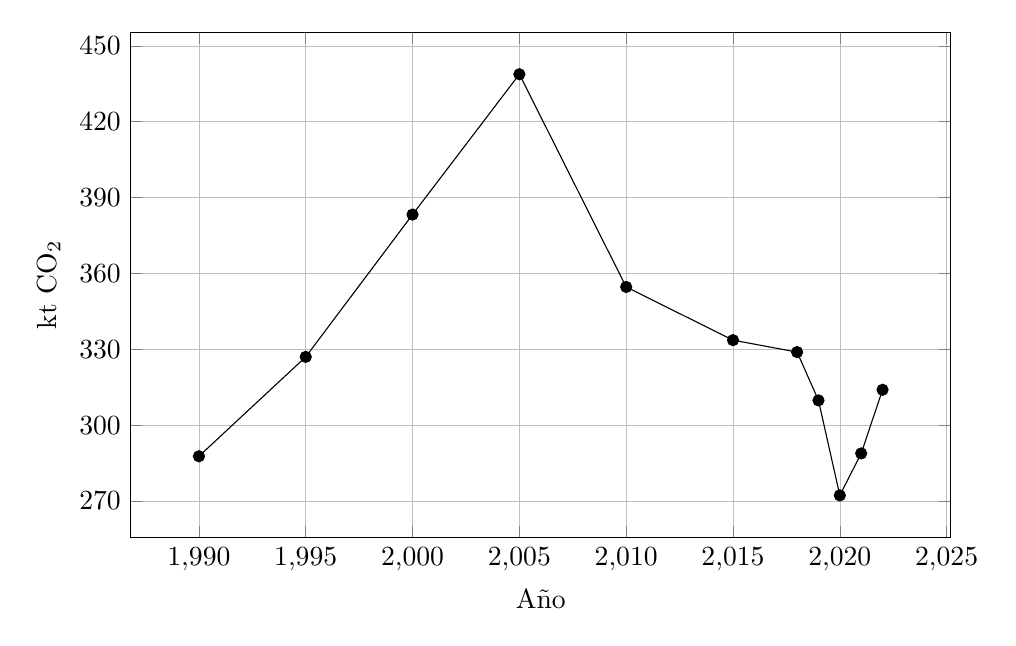
\begin{tikzpicture}
		\begin{axis}[
			xlabel={Año},
			ylabel={kt CO\textsubscript{2}},
			xtick={1990,1995,2000,2005,2010,2015,2020,2025},
			ytick={270, 300, ..., 450},
			grid=both,
			grid style={line width=.1pt, draw=gray!10},
			major grid style={line width=.2pt,draw=gray!50},
			width=12cm,
			height=8cm,
			]
			\addplot[mark=*] coordinates {
				(1990, 287.710)
				(1995, 327.011)
				(2000, 383.276)
				(2005, 438.760)
				(2010, 354.652)
				(2015, 333.623)
				(2018, 328.905)
				(2019, 309.814)
				(2020, 272.244)
				(2021, 288.848)
				(2022, 314.000)
			};
		\end{axis}
	\end{tikzpicture}

\end{figure}

En cuanto a las emisiones asociadas a la generación eléctrica:
\begin{table}[H]
	\centering
	\begin{tabular}{p{3cm}l*{11}{c}}
		\toprule
		tCO\textsubscript{2} $\times$ 1.000.000& 2011 & 2012 & 2013 & 2014 & 2015 & 2016 & 2017 & 2018 & 2019 & 2020 & 2021 & 2022 \\
		\midrule
		Carbón &   41,0 & 51,1 & 37,5 & 41,1 & 50,0 & 35,4 & 42,8 & 36,0 & 12,4 & 4,9 & 4,9 & 7,5 \\
		Fuel + Gas  &  0,0 & 0,0 & 0,0 & 0,0 & 0,0 & 0,0 & 0,0 & 0,0 & 0,0 & 0,0 & 0,0 & 0,0 \\
		Motores diésel &  2,9 & 2,9 & 2,7 & 2,6 & 2,7 & 2,8 & 2,7 & 2,2 & 2,0 & 1,6 & 1,7 & 1,7 \\
		Turbina de gas &  0,9 & 1,0 & 0,7 & 0,8 & 0,7 & 0,5 & 0,7 & 1,0 & 0,7 & 0,4 & 0,5 & 0,7 \\
		Turbina de vapor &  2,3 & 2,4 & 2,2 & 1,8 & 2,0 & 2,3 & 2,4 & 2,2 & 2,0 & 1,3 & 1,0 & 1,1 \\
		Ciclo combinado  & 21,0 & 16,4 & 11,4 & 10,5 & 12,0 & 12,0 & 14,9 & 11,8 & 21,2 & 17,1 & 17,4 & 26,2 \\
		Cogeneración  &  11,6 & 12,3 & 11,7 & 9,2 & 9,6 & 9,8 & 10,7 & 11,0 & 11,3 & 10,1 & 9,7 & 6,6 \\
		Residuos no renovables &  0,3 & 0,4 & 0,4 & 0,5 & 0,6 & 0,6 & 0,6 & 0,6 & 0,5 & 0,7 & 0,8 & 0,6 \\
		Total Emisiones &  80,1 & 86,4 & 66,6 & 66,5 & 77,6 & 63,5 & 74,9 & 64,9 & 50,0 & 36,1 & 35,9 & 44,4 \\ 
		\\
		\hline
		\\
		Factor de emision de CO\textsubscript{2} (tCO\textsubscript{2}/MWh) &  0,29 & 0,31 & 0,24 & 0,25 & 0,29 & 0,24 & 0,29 & 0,25 & 0,19 & 0,15 & 0,14 & 0,16 \\
		\bottomrule
	\end{tabular}
\end{table}

En cuanto a los rendimientos de diversas plantas de generación eléctrica:
\begin{table}[h]
	\label{tab:conversion-efficiency}
	\begin{tabular}{lcccc}
		\toprule
		&Eficiencia conversión&\multicolumn{3}{c}{Emisiones en gramos/kWh} \\
		\cline{3-5}
		&  (\%) & NOx & SO2 & CO2 \\
		\midrule
		Carbón pulverizado (sin descontaminar S) & 36 & 1.29 & 17.2 & 884 \\
		Carbón pulverizado (con descontaminación S) & 36 & 1.29 & 0.86 & 884 \\
		Carbón en lecho fluidificado & 37 & 0.42 & 0.84 & 861 \\
		Ciclo combinado de carbón gasificado & 42 & 0.11 & 0.3 & 758 \\
		Turbina de gas & 39 & 0.23 & 0 & 470 \\
		Ciclo combinado de turbina de gas & 53 & 0.1 & 0 & 345 \\
		\bottomrule
	\end{tabular}
\end{table}
\newpage
\section{Protocolo de Kioto.}
El Protocolo de Kioto estableció 3 vías para su cumplimiento:
\subsection{Políticas y medidas.}
Directiva 2033/87 CE de Comercio de Derechos de Emisión de gases
de efecto invernadero en la Unión Europea.
\subsection{Creación de sumideros.}
Se consideran sumideros todos los sistemas por los que se extraen gases de la atmósfera. Se consideran sumideros actividades como la reforestación.
\subsection{Mecanismos flexibles.}
\begin{enumerate}
	\item \textbf{Comercio de derechos de emisión (CDE):}
		Establece una asignación de una determinada cantidad de derechos de emisión gratuitos para
		las centrales térmicas y el sector industrial que equivalen a 1 tonelada de CO$_2$. Un país que haya conseguido reducir sus emisiones podrá vender a otro país que no llegue a su objetivo previsto. En España se llama \textbf{PNA} (Plan Nacional de Asignación).
	\item \textbf{Mecnismo de desarrollo limpio (MDL):}
		El país desarrollado invierte en tecnologías limpias en países en vías de desarrollo.
	\item \textbf{Aplicación conjunta (AC):}
		Un país desarrollado invierte en otro país desarrollado en un proyecto de energía limpia.
\end{enumerate}
\section{PNA.}
	La Directiva de la Unión Europea sobre Comercio de Emisiones (2003/87/CE) establece que cada Estado
	miembro deberá elaborar un Plan Nacional de Asignación (PNA) en el que se determinen la cantidad total de
	derechos a asignar durante un periodo y el procedimiento de asignación aplicado.
	
	
	Actualmente en España se asigna mediante el PNA IV donde se permiten unas emisiones de CO$_2$ = 44 MtCO$_{2-eq}$
\section{Precio de emisión.}
SENDECO2 es la plataforma que proporciona a todos los empresarios un lugar donde intercambiar Derechos de Emisión (EUAs) por Créditos de carbono (CERs) que certifican que se deja de emitir una tonelada de CO$_2$.
\subsection{Evolución del precio del derecho de emisión.}
\begin{figure}[H]
	\centering
	\includegraphics[width=1\linewidth]{res/tema2/precioEUA}
	\label{fig:t-emisiones}
\end{figure}
\newpage
\subsection{Influencia coste de emisión en el mercado eléctrico.}
Desde el año 2021 las centrales térmicas no tienen cantidades asignadas gratuitas y por ello, tienen que comprar derechos de emisión. Este coste repercute en el coste de la generación ofertado y, por tanto el precio de la energía como se puede ver en la figura inferior.
\begin{figure}[H]
	\centering
	\includegraphics[width=1.2\linewidth]{res/tema2/variacionPrecio}
	\label{fig:variacionprecio}
\end{figure}
\subsection{Factor de emisión.}
El factor de emisión (fe) representa la cantidad de CO$_2$ que se genera por MWh de electricidad producida en bornes de la central:
\[fe=\frac{tCO_{2-eq}}{MWhe}=\frac{tCO_{2-eq}}{TJ}\]
Los factores de emisión se actualizan anualmente.
\subsection{Cálculo del factor de emisión.}
Para el cálculo se emplea la siguiente expresión:
\[f\left(\frac{tCO_2}{MWh}\right)=\frac{tCO_2}{TJ}\cdot\frac{3,6 TJ}{1000 MWh}\cdot\frac{100}{\eta}\]
\begin{enumerate}
	\item \textbf{Centrales térmicas de carbón:}
		El carbón es un combustible con un alto contenido en carbono y por ello genera una cantidad elevada de CO$_2$ por MWhe. El tep (tonelada equivalente petróleo) es una unidad para referir la energía con respecto a la obtenida con una tonelada de petróleo.
	\begin{table}[H]
		\centering
		\renewcommand{\arraystretch}{1.1}
		\begin{tabular}{cm{2cm}m{2cm}m{3cm}m{2cm}m{2cm}}
			\hline
			\textbf{Combustible} & \textbf{ktCO2/ktep} & \textbf{TJ/ktep} & \textbf{Factor de Emisión  combustible (tCO2/TJ)} & \textbf{Rendimiento eléctrico (\%)} & (tCO2/MWh)\\  
			\hline
			Hulla + Antracita nacional & 4,032 & 41,868 & 96,303 & 36\% & 0,96 \\
			Carbón importado           & 4,032 & 41,868 & 96,303 & 36\% & 0,96 \\
			Lignito negro              & 3,861 & 41,868 & 92,218 & 36\% & 0,92 \\
			Lignito pardo              & 3,983 & 41,868 & 95,132 & 36\% &0,95 \\ \hline
		\end{tabular}
	\end{table}
	
	\item \textbf{Centrales térmicas de ciclo combinado con gas natural:}
		Utilizan gas natural, un combustible con menor contenido en carbono que junto a su elevado rendimiento hace que tenga un menor factor de emisión.
		\begin{table}[H]
		\centering
		\renewcommand{\arraystretch}{1.1}
		\begin{tabular}{cm{2cm}m{2cm}m{3cm}m{2cm}m{2cm}}
			\hline
			\textbf{Combustible} & \textbf{ktCO2/ktep} & \textbf{TJ/ktep} & \textbf{Factor de Emisión  combustible (tCO2/TJ)} & \textbf{Rendimiento eléctrico (\%)} & (tCO2/MWh)\\  
			\hline
			Gas natural & 2,337 & 41,868 & 55,818 & 54\% & 0,37 \\
		 \hline
		\end{tabular}
	\end{table}
	\newpage
	\item \textbf{Centrales térmicas de fuel-gas:}
		Debido a su heterogeneidad se utilizan valores medios empíricos para este conjunto de centrales.
				\begin{table}[H]
			\centering
			\renewcommand{\arraystretch}{1.1}
			\begin{tabular}{cm{2cm}}
				\hline
				\textbf{Combustible}  & (tCO2/MWh)\\  
				\hline
				Gas natural & 0,77 \\
				\hline
			\end{tabular}
		\end{table}
	\item \textbf{Centrales hidráulicas, renovables y nuclear:}
		No emiten CO$_2$ para generar electricidad.
		\begin{table}[H]
			\centering
			\renewcommand{\arraystretch}{1.1}
			\begin{tabular}{cm{2cm}}
				\hline
				\textbf{Combustible}  & (tCO2/MWh)\\  
				\hline
				Centrales hidráulicas, renovables y nuclear & 0
				 \\
				\hline
			\end{tabular}
		\end{table}
	\item \textbf{Cogeneración:}
		Consiste en la producción combinada de calor y electricidad, lo que permite conseguir un rendimiento conjunto superior.
		\begin{table}[H]
			\centering
			\renewcommand{\arraystretch}{1.1}
			\begin{tabular}{cm{2cm}}
				\hline
				\textbf{Combustible}  & (tCO2/MWh)\\  
				\hline
				Cogeneración & 0,37
				\\
				\hline
			\end{tabular}
		\end{table}
	\item \textbf{Residuos:}
		Como existe una gran heterogeneidad en los combustibles empleados se toma un valor medio. En el caso de la biomasa su factor de emisión es nulo porque son neutros a nivel de emisiones. Además las emisiones de N$_2$O asociadas a los residuos no son significativas a nivel de cálculos del factor de emisión.
		\begin{table}[H]
			\centering
			\renewcommand{\arraystretch}{1.1}
			\begin{tabular}{cm{2cm}m{2cm}}
				\hline
				\textbf{Combustible} & \textbf{Rendimiento eléctrico (\%)} & (tCO2/MWh)\\  
				\hline
				Residuos &25\%& 0,24
				\\
					Biomasa &-& 0
				\\
				\hline
			\end{tabular}
		\end{table}
\end{enumerate}
\subsection{Emisiones en la combustión.}
Las fuentes de combustión que producen emisiones de CO$_2$ se calculan multiplicando el contenido de energía por un factor de emisión y oxidación (se asume igual a 1 el factor de oxidación).
\[\text{Emisiones CO}_2 = \text{Datos de la actividad} \times \text{Factor de emisión} \times \text{Factor de oxidación}\]

Los datos de actividad se expresan como el contenido de energía neto del combustible consumido [TJ] durante un periodo.
\[\text{Contenido de energía [TJ]}=\text{Combustible consumido [t o m$^3$]}\times \text{Poder calorífico combustible [TJ/t o TJ/m$^3$]}\]

El poder calorífico neto es un valor representativo de la energía liberada en la combustión en forma de calor. Esta magnitud tiene límite superior (PCS) e inferior (PCI) en función de la humedad del combustible.

\[[PCI]_s (kcal/kg)=[PCS]_s-597\cdot (9H+H_2O)\]
\begin{itemize}
	\item [-] H $\rightarrow$ \% de hidrógeno contenido en el combustible (base seca).
	\item [-] H$_2$O $\rightarrow$ \% de humedad del combustible.
\end{itemize}

\subsection{Emisiones evitadas con las energías renovables.}
Las energías renovables en España permitieron reducir la emisión de 55,6 millones de tCO$_2$ y cubrieron el 42,2\% de la demanda eléctrica.
\newpage
\section{Combustibles fósiles.}
\subsection{Combustible sólidos.}
\begin{enumerate}
	\item \textbf{Biomasa:}
		El combustible esta compuesto de materia vegetal que había sido creada a través de la fotosíntesis:
		\[6 CO_2 + 6 H_2O + 112 kcal/mol \rightarrow C_6 (H_2O)_6 + 6 O_2 ( Glucosa)\]
		Por tanto, la fotosíntesis fija al año 18.000 Mt de CO$_2$ y por tanto, quemar esta planta no produce más CO$_2$ que el que liberaría al morir por fermentación. De esta manera, se podría considerar renovable.
	\item \textbf{Carbón:}
		Es una roca de fácil combustión con aproximadamente el 50\% del peso en carbono. No obstante, en función del porcentaje de carbono cambia el poder calorífico:
		\begin{table}[H]
			\centering
			\renewcommand{\arraystretch}{1.1}
			\begin{tabular}{cccc}
				\hline
				&\textbf{Lignito} & \textbf{Hulla} & \textbf{Lignito}\\  
				\hline
			Densidad &  1,1-1,3&1,2-1,5  &1,4-1,8\\ 
			Humedad (\%) &20-50  &3-25  &3-5\\ 
			\% C & 27-31 &  37-86&89-98\\ 
			\% Volátiles &25-55  &25-50  &2-14\\ 
			PC (kcal/kg) &  2000-4000&3500-7500  &7000-8350\\ 
				\hline
			\end{tabular}
		\end{table}
		De manera general en función del tipo de carbón el combustible tiene distintas propiedades:
		\begin{enumerate}
			\item \textbf{Lignito:}
			posee un color parduzco o negro. Por lo general tiene un alto contenido en volátiles. El lignito
			negro, o carbón subbituminoso, es duro y su humedad está limitada.
			Los lignitos españoles son altamente sulfurosos. El lignito
			pardo es un carbón terroso, con alto contenido en humedad.
			\item \textbf{Hulla:}
			carbón bituminoso o carbón graso. Abarca una amplia variedad de carbones.
			Es más blando que la antracita. Arde con llama humeante y larga. Su aspecto varía desde el pardo oscuro hasta
			el negro. Son los carbones que presentan un mayor interés para la generación eléctrica.
			\item \textbf{Antracita:}
			también llamado carbón de piedra o carbón duro. De gran contenido en carbono fijo. Es duro y negro. Tiene lustre semimetálico y fractura semiconcoidal. Arde con llama azul y
			corta, sin apenas humo.
		\end{enumerate}
		El carbón esta formado por distintos elementos que condicionan su comportamiento como combustible:
		\begin{enumerate}
			\item \textbf{Carbón fijo (65-95\%):}
				A mayor porcentaje mayor poder calorífico. Permite estimar el porcentaje de generación de CO$_2$.
			\item \textbf{Hidrógeno (3-6\%):}
				Aumenta el poder calorífico y facilita la combustión.
			\item \textbf{Azufre (0,2-11\%):}
				Los carbones con alto contenido en azufre deben ser tratados porque generan SO$_2$ $\rightarrow$SO$_3$ que es altamente contaminante al provocar lluvias ácidas y ser peligroso para el ser humano.
				
				
				Los tratamientos normalmente empleados para reducir el porcentaje de azufre son:
				\begin{itemize}
					\item [-] Lavaderos de carbón: Antes de la combustión.
					\item [-] Adición de caliza: Durante la combustión (\textbf{solo lecho fluido y gasificación}).
					\item [-] Desulfuración de los gases: Después de la combustión.
				\end{itemize}
			\item \textbf{Humedad (1-60\%):}
				Provoca una disminución del poder calorífico y del rendimiento. Además necesita aire más caliente y puede provocar atascos en las tolvas.
			\item \textbf{Nitrógeno (1-1,5\%):}
				Provoca la formación de NOx en función de la temperatura de combustión.
			\item \textbf{Oxígeno (2-30\%):}
				Sirve como medida del grado de oxidación y permite reducir la cantidad de aire a aportar.
				\newpage
			\item \textbf{Materia volátil (5-40\%):}
				Se desprende durante la fase inicial del proceso de combustión, facilitan la ignición. A mayor materia volátil mayor será el humo producido.
				\begin{itemize}
					\item [-] Si tienen mucha materia volátil dan llamas cortas , calientes y muy estables. Hay pocos inquemados.
					\item [-] Si tienen poca materia volátil dan llamas largas e inestables. Se necesitan fuegos opuestos para elevar la temperatura de llama u hogares de arco que
					soporten llamas muy largas. Necesita molienda muy fina.
				\end{itemize}
			\item \textbf{Cenizas (30\%):}
				Materiales minerales no volátiles. Son residuos tras la combustión completa. Reducen la calidad del carbón.		
		\end{enumerate}
		\textbf{Combustión del carbón:} Es una reacción de oxidación con fuente de ignición donde el oxígeno se combina con el combustible para formar óxidos liberando gran cantidad de calor.
		\begin{itemize}
			\item [-] Para favorecer la combustión se pulveriza el carbón.
			\item [-] \textbf{Reacciones principales:}
			\[C+O_2\rightarrow CO_2 + 8100kcal/kg \ de \ C\]
			\[C+0,5O_2\rightarrow CO +2500kcal/kg \ de \ C\]
			\[H_2+0,5O_2\rightarrow H_2O +33600kcal/kg \ de \ H_2\]
			\[S+O_2\rightarrow SO_2 +2500kcal/kg \ de \ S\]
			\[N+O_2\rightarrow NO+O\]
			\item [-] \textbf{Condiciones necesarias combustión completa:}
			\begin{itemize}
				\item Cantidad suficiente de aire (con algo de exceso).
				\item Procurar buen grado de mezcla entre comburente y combustible (pulverización).
				\item Tiempo de residencia suficiente.
				\item Garantizar temperatura mínima en el hogar.
			\end{itemize}
			\item [-] Se considera que la combustión tiene lugar cuando la velocidad de oxidación es suficiente como para automantenerse. Cuando la velocidad de alimentación del combustible y comburente iguala a la velocidad de
			propagación de la llama entonces se estabiliza.
			\item [-]La caldera más común es la de carbón pulverizado. El diseño de estas depende del carbón a quemar.
			\begin{itemize}
				\item 240 minutos para plena carga en arranque en frío.
				\item 120 minutos para plena carga en arranque en templado (24h parada).
				\item 70 minutos para plena carga en arranque en caliente (8h parada).
				\item 60 minutos para plena carga en rearranque (2h parada).
			\end{itemize}
			\item [-] \textbf{Tipos de combustiones:} Desde el punto de vista estequiométrico puede ser completa o incompleta.
			\begin{itemize}
				\item Se considera completa cuando el combustible no quemado no supera el 2\%.
				\begin{itemize}
					\item 13 Nm$^3$ de aire por kg de carbono.
				\end{itemize}
				\item En la combustión incompleta se emite CO.
			\end{itemize}
			Se controla el tipo de combustión mediante la medida de gases a la salida de la chimenea.
			\begin{itemize}
				\item Índice emisión: 
				\[EI=\frac{\text{masa de gases emitidos}}{\text{masa de combustible quemado}}\]
				\item Masa de contaminante emitida por unidad de combustible quemado: 
				\[M/ud= \frac{EI}{Hc} (gr/MJ)\]
				\item Indice inmisión: emisión a 2m de altura sobre el suelo.
			\end{itemize}
			\item [-] \textbf{Combustión con exceso de aire:}
				Para evitar la formación de inquemados sólidos se procura una mezcla homogénea y se introduce un exceso de caudal. Para ello, se definen el exceso de aire porcentual (EA) y el coeficiente de exceso de aire (n):
				\[EA(\%)=100\times\frac{A_{exp}-A_{teórico}}{A_{teórico}}=100\times(n-1)\]
				No obstante, aumentar demasiado el exceso de aire provoca que se pierda parte del calor de la caldera.
				\begin{table}[H]
					\centering
					\renewcommand{\arraystretch}{1.1}
					\begin{tabular}{cc}
						\hline
						\textbf{Combustible}&\textbf{n}\\  
						\hline
						Gaseoso& 1,1-1,2\\
						Líquido & 1,15-1,3\\
						Pulverizado & 1,15-1,5\\ 
						\hline
					\end{tabular}
				\end{table}
				Para conocer el exceso de aire a emplear se emplea el diagrama de Oswald a partir de los contenidos de CO y CO$_2$. La región de trabajo óptima se situa en torno al 13\% de CO$_2$ en los gases de combustión.
				\begin{figure}[H]
					\begin{minipage}{0.6\linewidth}
						\centering
						\includegraphics[width=\linewidth]{res/tema2/oswaldo}
						\label{fig:oswaldo}
					\end{minipage}%
					\begin{minipage}{0.4\linewidth}
						\centering
						\includegraphics[width=\linewidth]{res/tema2/CO2O2}
						\label{fig:co2o2}
					\end{minipage}
				\end{figure}
				\item [-] \textbf{Balance energético en la caldera:} Se deben tener en cuenta las características energéticas y gasto del combustible frente a la calidad del vapor generado.
				
				
				Las principales pérdidas de calor en la caldera se deben a:
				\begin{itemize}
					\item Combustión incompleta: Se reduce a medida que se aumenta el exceso de aire.
					\item Calor sensible de los gases de escape: Aumenta a medida que se aumenta el exceso de aire.
					\item Sólidos inquemados: Disminuye a medida que se aumenta el exceso de aire.
				\end{itemize}
				Que resumido en un gráfico queda:
				\begin{figure}[H]
					\centering
					\includegraphics[width=0.6\linewidth]{res/tema2/perdidas}
					\label{fig:perdidas}
				\end{figure}
				Por tanto, el rendimiento de la caldera queda como:
				\[\eta = \frac{\text{Potencia térmica cedida al vapor sobrecalentado de salida}}{PCI \times \dot{m}_\text{combustible} \times \text{Potencia térmica aire caliente}}\approx 85-88\%\]
		\end{itemize}
\end{enumerate}
\subsection{Combustible gaseosos.}
\subsection{Combustible líquidos.}